\documentclass[12pt]{article}
\usepackage{amsmath}
\usepackage{amssymb}
\usepackage{graphicx}
\usepackage{physics}
\usepackage{siunitx}
\usepackage{wrapfig}

\AtBeginDocument{\RenewCommandCopy\qty\SI}
\newcommand{\E}[1]{\times 10^{#1}}

\begin{document}
    \section{Problem 1}
        (8 points) System A is at $40\unit{\celsius}$ and system B is at $0\unit{\celsius}$. 
        The two systems are connected by a sequence of rods with conductances $K_1 = 100 \unit{\watt/\kelvin}$, $K_2 = 125 \unit{\watt/\kelvin}$ and $K_3 = 175 \unit{\watt/\kelvin}$, as shown below.
        \begin{center}
            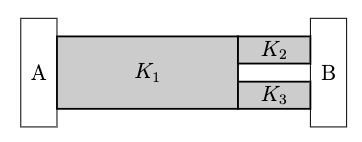
\includegraphics{picture_1.png}
        \end{center}

        Calculate the rate of heat flow through each rod and the temperature in the middle where $K_1$ is connected to the parallel combination of $K_2$ and $K_3$.

        \subsection{Solution}
            The best move here would be to calculate the equivalent heat conductence of the entire system.
            \begin{align}
                K_{23}  &=  K_2 + K_3\\
                K_{\rm eq}  &=  \left( \frac{1}{K_1} + \frac{1}{K_2 + K_3} \right)^{-1}
            \end{align}

            This can be multiplied by the change in temperature to get the heat flow along the entire system.
            \begin{align}
                \Delta T    &=  -40\unit{\kelvin}\\
                \dv{Q}{t}   &=  K \cdot \Delta T
                    =   \left( \frac{1}{K_1} + \frac{1}{K_2 + K_3} \right)^{-1} * \Delta T\\
                    &=  \left( \frac{1}{100} + \frac{1}{125 + 175} \right)^{-1} * (-40)
                    =   -3000\,\unit{\watt}
            \end{align}

            Since heat flows 

            This would equivalently be the rate at which the heat would flow through rod $K_1$, as well as the combination of rods two and three.
            It can also be first used to find the temperature at where $K_1$ is connected.
            \begin{align}
                \Delta T    &=  \frac{dQ/dt}{K_1}
                    =   \frac{-3000}{100}
                    =   -30\,\unit{\kelvin}\\
                T_{\rm middle}  &=  40\unit{\celsius} - 30\,\unit{\kelvin}
                    =   10\,\unit{\celsius}
            \end{align}

            This equivalently makes $\Delta T$ between the middle and system B equal to $-10\,\unit{\kelvin}$. 
            This in turn can be used to find the rate of heat flow along both $K_2$ and $K_3$.
            \begin{align}
                \left( \dv{Q}{t} \right)_2  &=  K_2 * \Delta T
                    =   125 * (-10)
                    =   -1250\,\unit{\watt}\\
                \left( \dv{Q}{t} \right)_3  &=  K_3 * \Delta T
                    =   175 * (-10)
                    =   -1750\,\unit{\watt}
            \end{align}

    \pagebreak
    \section{Problem 2}
        2. (2 points) A particular system executes a cyclical process whose P-V graph is a clockwise-directed ellipse centered at ($V_0$, $P_0$) and radii $\delta V$ and $\delta P$, respectively. 
        Calculate the net work done and the net heat flow into/out of this system during one cycle.
        \begin{center}
            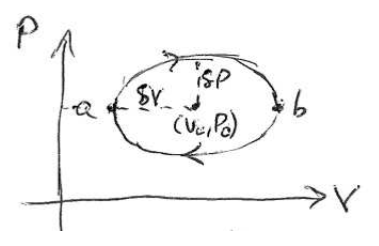
\includegraphics{picture_2.png}
        \end{center}

        \subsection{Solution}
            We know that the process is cyclical, so the net change in internal energy will be zero. 
            This, due to the first law of thermodynamics, means that the heat inserted is equal to the negative of the work done on the system, so we only have to calculate one of the two.
            To do this, we can set up an equation for the work done on the system.
            \begin{align}
                W   &=  -\int_{t_i}^{t_f} P(t)\,\dv{V(t)}{t}\,dt
            \end{align}

            There is an equation for the ellipse.
            \begin{gather}
                \frac{\left( V(t) - V_0 \right)^2}{\delta V^2} + \frac{\left( P(t) - P_0 \right)^2}{\delta P^2} = 1
            \end{gather}

            We can use ths to solve for $V(t)$.
            \begin{gather}
                \frac{\left( V(t) - V_0 \right)^2}{\delta V^2} + \frac{\left( P(t) - P_0 \right)^2}{\delta P^2} = 1\\
                \frac{\left( V(t) - V_0 \right)^2}{\delta V^2} = 1 - \frac{\left( P(t) - P_0 \right)^2}{\delta P^2}\\
                \left( V(t) - V_0 \right)^2 = \delta V^2 \left( 1 - \frac{\left( P(t) - P_0 \right)^2}{\delta P^2} \right)
            \end{gather}

\end{document}